\chapter{Aktueller Stand der Forschung und Praxis (generell auch wiedergeben von aktuell existierenden Lösungsmustern)}

\section{Ressourcenverbrauch bei KI-Modellen}
\subsection{Ressourcenverbrauch bei KI-Modellen}
\subsubsection{Nachhaltigkeit}
\subsubsection{Stromverbrauch}
\subsubsection{Rechenleistung begrenzt, KI-Modelle wachsen schneller als verfügbare Leistung}

\section{Deep Neural Network - Boltzmann Maschinen (Erstmal DNN erklären generell)}

(Erklären von Deep Neurol Network und Neurol Network) -> Anwendungsbereiche Spracherkennung, Image recognition
Solche Deep Neural Networks, sind sehr ressourceneffizient und möglicher Forschungsbereich für Nutzung des Hardwarebeschleunigers
Idee dabei, die repräsentationspower von energybased model höher als bei LLMs, mit weniger Neuronen besser als LLMs 


Some regression tasks within computer vision in \ac{DNN} include object detection, medical image registration, head- and body-pose estimation, age estimation and visual tracking.\footcite[Vgl.][325-326]{gustafssonEnergyBasedModelsDeep2020}


Energy Based Models -> Hinton Paper Gleichung 2, Warscheinlichkeitsbasierte Modelle
Durch Gleichung 3 kann erklärt werden wieso es nicht berechenbar ist. 

-> Dann auf BM kommen und erklären mit Training 

->RBMs einführen und sagen warum Training vereinfacht ist

\subsection{Energy-based models}


An \ac{EBM} is a type of statistical model where the likelihood of a particular state is determined by an energy function.\footcite[Vgl.][2]{huembeliPhysicsEnergybasedModels2022}
Since 1982, those models have been continuously emerging in the machine learning field when J.J. Hopfield introduced the Hopfield Network.\footcite[Vgl.][]{hopfieldNeuralNetworksPhysical1982}
Current developments include their use in reinforcement learning, potential replacements for discriminators in generative adversarial networks and for quantum \ac{EBM}s.\footnote{Vgl.\cite{verdonQuantumHamiltonianBasedModels2019}, p. 1; Vgl.\cite{duModelBasedPlanning2021}, p. 1}
The underlying idea behind \ac{EBM}s is to establish a probabilistic physical system that is able to learn and memorize patterns but most importantly generalize it.\footcite[Vgl.][2]{huembeliPhysicsEnergybasedModels2022} 
Specifically it involes learning an energy function \(E_{\theta}(x) \in \mathbb{R}\) and assigning the low energy to the observed data \(x_i\) and high energy to other values \(x\).\footcite[Vgl.][330]{gustafssonEnergyBasedModelsDeep2020}
The total energy \( E(x) \) of any given state of the system can be expressed through the following equation: 
\begin{equation}
    E(x) = \sum_i \theta_i f_i(x),
\end{equation}
for the parameters $\theta_i$ and functions $f_i(x)$.\footcite[Vgl.][3]{hintonPracticalGuideTraining2012}
The \ac{EBM} works by coming up with a specific parameterization of the negative log probability, which is called energy, and then computing the density with a proper normalization\footcite[Vgl.][2]{zhaiDeepStructuredEnergy2016}
These models are commonly trained by minimizing the negative log-likelihood, stemming from the probabilistic model:
\begin{equation}
    P(x) = \frac{1}{Z} \exp\left(-\frac{E(x)}{T}\right),
\end{equation}
with association to the instance \( Z \) 
that is given by the partition function to ensure that the density function normalizes to a total probability of 1.\footcite[Vgl.][2]{zhaiDeepStructuredEnergy2016}
The `partition function', \( Z \), is given by summing over all possible pairs of visible and hidden vectors:
\begin{equation}
    Z = \sum_x \exp\left(-\frac{E(x)}{T}\right)
\end{equation}

It is worth mentioning that using the maximum likelihood estimator for \( Z \) is impractical due to the requirement of summing over all possible states, which leads to an exponential increase in the number of states for larger systems.\footcite[Vgl.][2-3]{zhaiDeepStructuredEnergy2016}


\subsection{Konzept und Anwendung des Modells}

A \ac{BM} is a symmetrical energy-based network consisting of neurons.\footcite[Vgl.][260]{amariInformationGeometryBoltzmann1992}
The neurons of the network can be split into two functional groups, a set of visible neurons and a set of hidden neurons.\footcite[Vgl.][154]{ackleyLearningAlgorithmBoltzmann1985}
Therefore, the \ac{BM} is a two-layer model and has a visible layer (``v'') and a hidden layer (``h'').\footcite[Vgl.][448]{salakhutdinovDeepBoltzmannMachines2009}
The visible layer is the interface between the network and the environment. It receives data inputs during training and sets the state of a neuron to either {0; 1} which represents activated or not activated.
On the other hand, the hidden units are not connected to the environment and can be used to “explain” underlying constraints in the ensemble of input vectors and they cannot be represented by pairwise constraints.\footcite[Vgl.][154]{ackleyLearningAlgorithmBoltzmann1985}
The connection between the individual neurons is referred to as bidirectional, as each neuron communicates with each other in both directions.\footcite[Vgl.][149]{ackleyLearningAlgorithmBoltzmann1985}
In the following figure \ref{fig1}, a general \ac{BM} is depicted, where the upper layer embodies a vector of stochastic binary 'hidden' features, while the lower layer embodies a vector of stochastic binary 'visible' variables.\footcite[Vgl.][449]{salakhutdinovDeepBoltzmannMachines2009}

\begin{figure}[H]
    \centering
    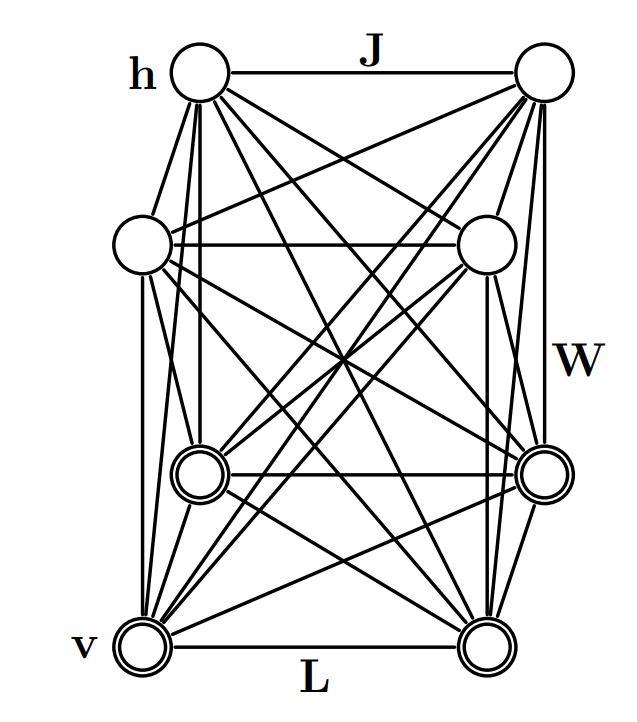
\includegraphics[width=0.25\linewidth]{graphics/General_BM.png}
    \caption{Figure of a general \ac{BM}}
    \label{fig1}
\end{figure}

It contains a set of visible units \( v \in \{0, 1\}^D \), and a set of hidden units \( h \in \{0, 1\}^P \) (see Fig. 1). The energy of the state \( \{v, h\} \) is defined as:

\begin{equation}
E(v, h; \theta) = -\frac{1}{2} v^T L v - \frac{1}{2} h^T J h - v^T W h
\end{equation}

where \( \theta = \{W, L, J\} \) are the model parameters.\footcite[448][Vgl.]{salakhutdinovDeepBoltzmannMachines2009}
\( W, L, J \) represent visible-to-hidden, visible-to-visible and hidden-to-hidden weights.
 

The network can update the weights ``W'' that exist between the neurons through specific training rules based on the observations that served as input.\footcite[Vgl.][1-2]{barraEquivalenceHopfieldNetworks2012}

As early as 1985, one of the founding fathers of artificial intelligence, ``Geoffrey Hinton'', was aware that an \ac{BM} is able to learn its underlying features by looking at data from a domain and developing a generative internal model.\footcite[Vgl.][148]{ackleyLearningAlgorithmBoltzmann1985}
In the next step, it is possible to generate examples with the same probability distribution as the examples shown.


\subsection{Energiefunktion, Training von BMs}


If the diagonal elements \( L \) and \( J \) of the general \ac{BM} introduced earlier, are set to 0 the known model of a \ac{RBM} establishes shown in fig.2.\footcite[Vgl.][449]{salakhutdinovDeepBoltzmannMachines2009}

\begin{figure}[H]
    \centering
    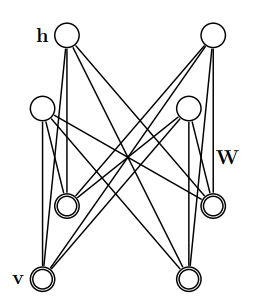
\includegraphics[width=0.25\linewidth]{graphics/RBM_Modell.png}
    \caption{Figure of a \ac{RBM}}
\end{figure}
As a result no more visible-to-visible and hidden-to-hidden connections can be found in the network.
The configuration of the visible and hidden units \( (v, h) \) has an energy (Hopfield, 1982) given by:
\begin{equation}
E(v, h) = - \sum_{i \in \text{visible}} a_i v_i - \sum_{j \in \text{hidden}} b_j h_j - \sum_{i,j} v_i h_j w_{ij}
\end{equation}

where \( v_i, h_j \) are the binary states of visible unit \( i \) and hidden unit \( j \), \( a_i, b_j \) are their biases and \( w_{ij} \) is the weight between them.\footcite[Vgl.][3-4]{hintonPracticalGuideTraining2012a}

\subsection{Restriced Boltzmann Machine}


\subsubsection{Markov-Chain-Monte-Carlo-Verfahren}
Metropolis Hastings,
Conrtrastive Divergence

\subsection{Aktuelle Probleme mit RBM/BM}


Exact maximum likelihood learning in the Boltzmann machine is infeasible due to the exponentially increasing computation time with the number of hidden units.
Hinton and Sejnowski's 1983 algorithm approximates this via Gibbs sampling, but it is limited by the significant time needed to reach the stationary distribution in a complex, multimodal energy landscape.

\section{Hardwarebeschleuniger}
\subsection{Aktuelle Ansätze im Bereich KI und weitere Lösungen}
\subsubsection{Asics}
\subsubsection{Quantencomputing}
\subsection{ISING Maschine/ Physikinspirierter Hardwarebeschleuniger}
\subsubsection{Konzept (mit Energiefunktion), Probleme der Digitalrechner bzw. Unterschied zu Digitalrechner}
\subsubsection{Aktuelle Anwendung}
\subsubsection{Potentielle Einsatzgebiete für KI-Modelle}
\subsubsection{Parallelen Energiefunktion BM und ISING Maschine}

\section{Memristor Hopfield Network}
\subsection{Memristor}
\subsection{Hopfield Network}
\subsection{Crossbar}
\subsection{Output Hopfield Networtk}
\subsection{Noisy HNN}
